% !TEX root = CartaPerali_Report.tex

\section{Results}
\label{sec:results}
\noindent In this section the test results are presented. The confusion matrix in Figure. \ref{fig:conf_matrix_cnn} shows the affective ability of the model in making predictions.

\begin{figure}[h]
			\centering
	    	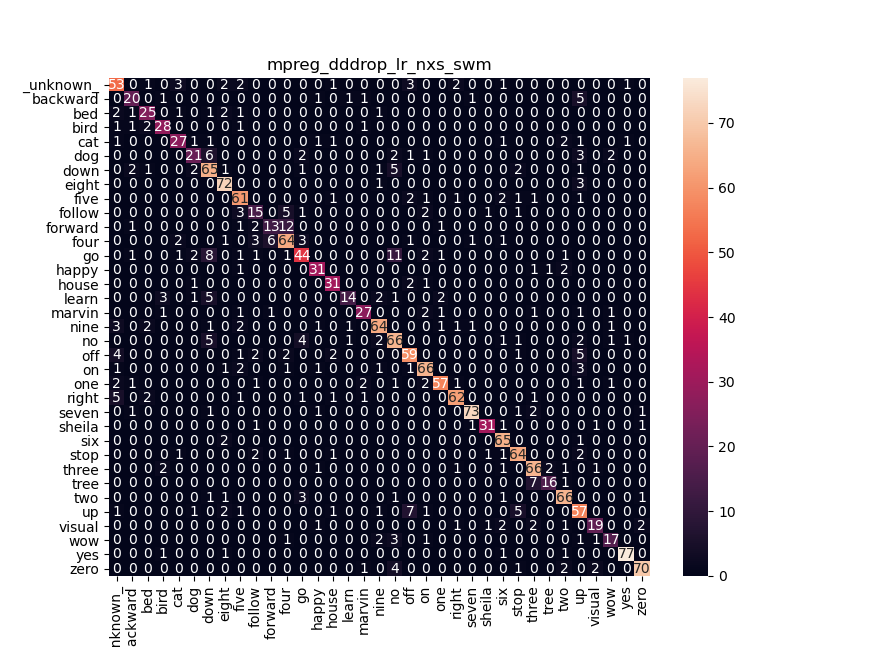
\includegraphics[width=10cm, height=8cm]{conf_matrix_cnn_dii_cm}
	    	\caption{Confusion matrix}
	    	\label{fig:conf_matrix_cnn}
\end{figure} 

\begin{table*}[ht]
	\centering
	\begin{tabular}{|c c c c c c c c|}
		\hline
		Configuration & Preprocessing type & Optimizer & Learning rate & Trainable parameters & Epochs  & Labels & Accuracy \\
		\hline
		A &Specgram&Adam&5e-4&&10&35&80.3\% \\
		B &Specgram&Adam&1e-4&&20&35&79.2\% \\
		C &Specgram&Adam&5e-5&&25&35&78.9\% \\
		\hline
	\end{tabular}
	\caption{Preprocessing}
	\label{table:Pr_eprocessing}
\end{table*}



\noindent From the above results we can observe how {\red{to be continued...}}